
En la figura \ref{fig:TopicDetectionDiag} se presenta la metodología propuesta para resolver la tarea de detección de tópicos a través de una representación de palabras con modelos profundos y técnicas de \textit{clustering}. Esta metodología se inspiro principalmente en el trabajo presentados en \cite{DeepRepresentationClusteringTweets}, en donde no solo se utiliza el modelo BERT para hacer la representación de las palabras sino que esto combina con un \textit{autoencoder} para reducir la dimensionalidad de las representaciones. No obstante, dadas las limitaciones de computación y de tiempo, no se utilizaron las representaciones de todas las palabras, ni un autoencoder basado en redes convolucionales 2D, sino que se implementó una aproximación más sencilla del mismo modelo, la cual se explica más adelante en esta sección. Asimismo, para poder hacer una descripción de los tópicos (resultado de las agrupaciones hechas por el algoritmo de \textit{clustering}), se tomaron ideas de \cite{TrendTopicsDetectionFromTwitter}, al buscar las palabras claves de cada \textit{cluster} y representarlas en una nube de palabras. Finalmente, se hizo un análisis de estos resultados a nivel de las agrupaciones obtenidas y el comportamiento a lo largo del tiempo, lo cual permitió ajustar los parámetros de cada una de las distintas etapas de procesamiento y obtener resultados presentados.

\begin{figure}[H]
    \centering
    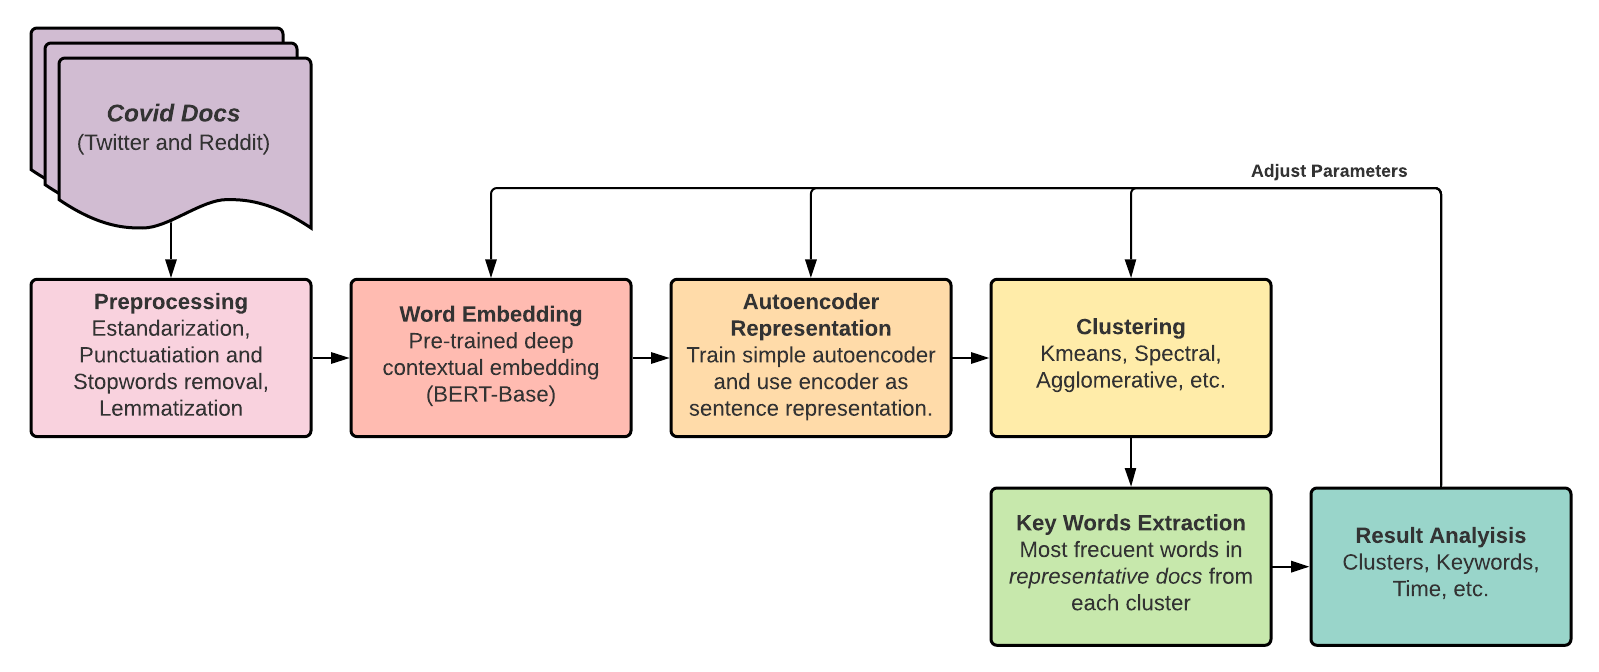
\includegraphics[width=\textwidth]{doc_hw04/images/TopicDetectionDiag.png}
    \caption{Metodología propuesta para la detección de tópicos utilizando \textit{deep sentence representation} y \textit{clustering}.}
    \label{fig:TopicDetectionDiag}
\end{figure}

\subsection{Dataset}
El \textit{dataset} utilizado para detección de temas en tendencia corresponde documentos recogidos por los autores de dos fuentes diferentes \textit{Twitter} y \textit{Reddit} en inglés, español y francés. Por cuestión de tiempo de procesamiento se decidió excluir las noticias recopiladas. Si bien se tiene una gran cantidad de datos en inglés (más de 800.00 documentos) se decide utilizar únicamente alrededor de 135.000 datos con el fin de impedir que la cantidad de documentos favoreciera un idioma por encima de otro, y poder analizar con mayor imparcialidad. El total de documentos utilizados en cada caso se muestra en la tabla \ref{tab:docs}.

\begin{table}[H]
\centering
\caption{Total de documentos utilizados por idioma}
\label{tab:docs}
\begin{tabular}{lrrrr}
\hline
\textbf{Idioma} & \textbf{Twitter} & \textbf{Reddit} & \textbf{Total} \\ \hline
Inglés          & 99.971           & 45.725          & 145.696        \\
Español         & 125.000          & 6.479           & 131.479        \\
Francés         &                  &                 &                \\ \hline
\end{tabular}
\end{table}

\subsection{Preprocesamiento}

El preprocesamiento de los datos se realizó siguiendo los siguientes pasos:
\begin{enumerate}
    \item Pasar todas las palabras a minúsculas.
    \item Eliminar signos de puntuación y caracteres especiales.
    \item Tokenizar las palabras.
    \item Lematizar las palabras.
\end{enumerate}

\begin{itemize}
    \item \textbf{Reddit original:}
    \begin{itemize}
        \item [\textbf{Inglés:}] Someone I am close to works in a factory called Dixon in Maryland. This person is one of only 2 people wearing a mask in the entire factory, including office staff. How this is acceptable I have no idea. The recklessness and denial in the face of a global pandemic is astounding. Companies not protecting employees in close proximity with masks wearing policy should be fined. It's criminal given what we know about transmission.
        \item [\textbf{Español:}] INER está al 100\% de capacidad por COVID y personal está agotado, advierte su director.
        \item [\textbf{Francés:}] Pourquoi autant mentir? On veut freiner et éliminer la contagion au Québec ou la nourrir comme on arrose un jardin? Je comprends pas.
    \end{itemize}
    \item \textbf{Reddit preprocesado:}
    \begin{itemize}
        \item [\textbf{Inglés:}] 'someone', 'close', 'works', 'factory', 'called', 'dixon', 'maryland', 'person', 'one', '2', 'people', 'wearing', 'mask', 'entire', 'factory', 'including', 'office', 'staff', 'acceptable', 'idea', 'recklessness', 'denial', 'face', 'global', 'pandemic', 'astounding', 'companies', 'protecting', 'employees', 'close', 'proximity', 'masks', 'wearing', 'policy', 'fined', 'criminal', 'given', 'know', 'transmission'
        \item [\textbf{Español:}]'iner', '100', 'capacidad', 'covid', 'personal', 'agotado', 'advierte', 'director'.
        \item [\textbf{Francés:}] 'pourquoi', 'autant', 'mentir', 'veut', 'freiner', 'éliminer', 'contagion', 'québec', 'nourrir', 'comme', 'arrose', 'jardin', 'comprends'
    \end{itemize}
    \item \textbf{Tweet original:}
    \begin{itemize}
        \item [\textbf{Inglés}] \#WorldBank “Living paper”: \#SocialProtection and Jobs - Responses to \#COVID19: A Real-Time Review of Country Measures; version 15 (May 14, 2021)
        \item [\textbf{Español:}] Madrid ha gastado ya, dicen aquí, 299 millones de euros en hacer frente a la pandemia... habiendo recibido 3.384 millones...
        \item [\textbf{Francés:}] La progression de la protection vaccinale contre la covid 19 permettra-t-elle prochainement d'assouplir les recommandations ? \#COVID19 \#VaccinationCovid 
    \end{itemize}
    \item \textbf{Tweet preprocesado:}\\ 
    \begin{itemize}
        \item [\textbf{Inglés:}] 'worldbank', 'living', 'paper', 'socialprotection', 'jobs', 'responses', 'covid19', 'realtime', 'review', 'country', 'measures', 'version', '15', 'may', '14', '2021'
        \item [\textbf{Español:}] 'madrid', 'gastado', 'dicen', 'aquí', '299', 'millones', 'euros', 'hacer', 'frente', 'pandemia', 'recibido', '3384', 'millones'
        \item [\textbf{Francés:}] 'progression', 'protection', 'vaccinale', 'contre', 'covid', '19', 'permettratelle', 'prochainement', 'dassouplir', 'recommandations', 'covid19', 'vaccinationcovid'
    \end{itemize}
\end{itemize}

\subsection{Extracción de características}

Una vez preprocesados los datos se procedió a extraer las características (\textit{o features}) de cada una de las sentencias utilizando un modelo profundo pre-entrenado. Para este trabajo se utilizaron en total 3 versiones de BERT-base pre-entrenadas, una para cada idioma: El modelo 
bertweet-covid19-base-uncased \cite{bertweet} (reentrenado sobre un corpus de 850M de tweets relacionados con las tematicas de covid-19), el modelo de BETO o Spanish BERT \cite{CaneteCFP2020} (reentrenado para idioma español) y finalmente el modelo bert-base-french-europeana-cased (reentrenado para idioma framces). Adicionalmente, se hicieron pruebas sobre el modelo covid-twitter-bert-v2 \cite{muller2020covid}, no obstante, al estar este basado en el BERT-Large, el tiempo de computo era considerablemente mayor por lo que fue necesario descartar dicha opción. \\

Ahora bien, de estos modelos es posible obtener varias representaciones a nivel de palabras o de sentencias con base en los distintos tokens que utiliza el modelo (véase figura \ref{fig:BERT_Tokens}). En este caso, se decidió utilizar como representación de la sentencia el token \texttt{CLS}. Este es un token especial utilizado en la tarea de clasificación y que codifica la información de toda la expresión, en este caso todo el documento (tweet,  post o comentario de Reddit). De esta manera, para cada documento se tendrá un vector asociado a su representación de 768 posiciones. 

\begin{figure}[H]
    \centering
    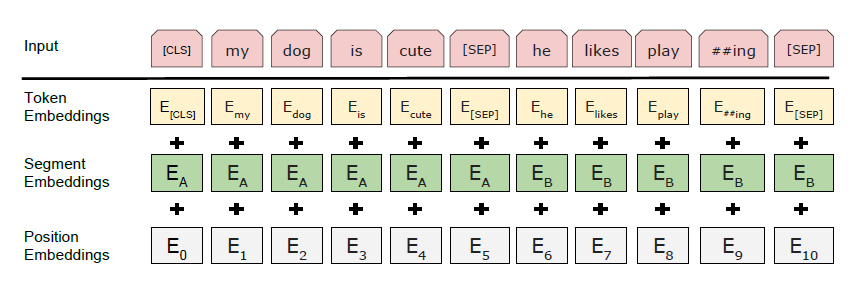
\includegraphics[width=0.8\textwidth]{doc_hw04/images/BERT_Tokens.png}
    \caption{\textit{Tokens} utilizados en el modelo BERT}
    \label{fig:BERT_Tokens}
\end{figure}

No obstante, los algoritmos de \textit{clustering} suelen presentar un mejor funcionamiento en espacios de dimensiones reducidas, esto mejora la convergencia pues da una mejor idea del concepto de distancia. Así las cosas y similar a como se presenta en \cite{DeepRepresentationClusteringTweets} se utiliza un autoencoder para reducir la dimensionalidad de las representaciones (véase figura \ref{fig:autoencoder}). El modelo utilizado no es más que una red neuronal que se entrena con los mismos datos a la entrada y a la salida, lo que internamente comprime y descomprime la información. Esto permite obtener una representación, en un espacio latente mucho menor al de la entrada (en este caso se paso de 768 a 32 dimensiones), que contiene suficiente información para reconstruir la misma información en la salida. Así las cosas, es esta información codificada la que se utilizó como entrada al modelo de agrupación o \textit{clustering} para realizar la detección no supervisada de tópicos.

\begin{figure}[H]
    \centering
    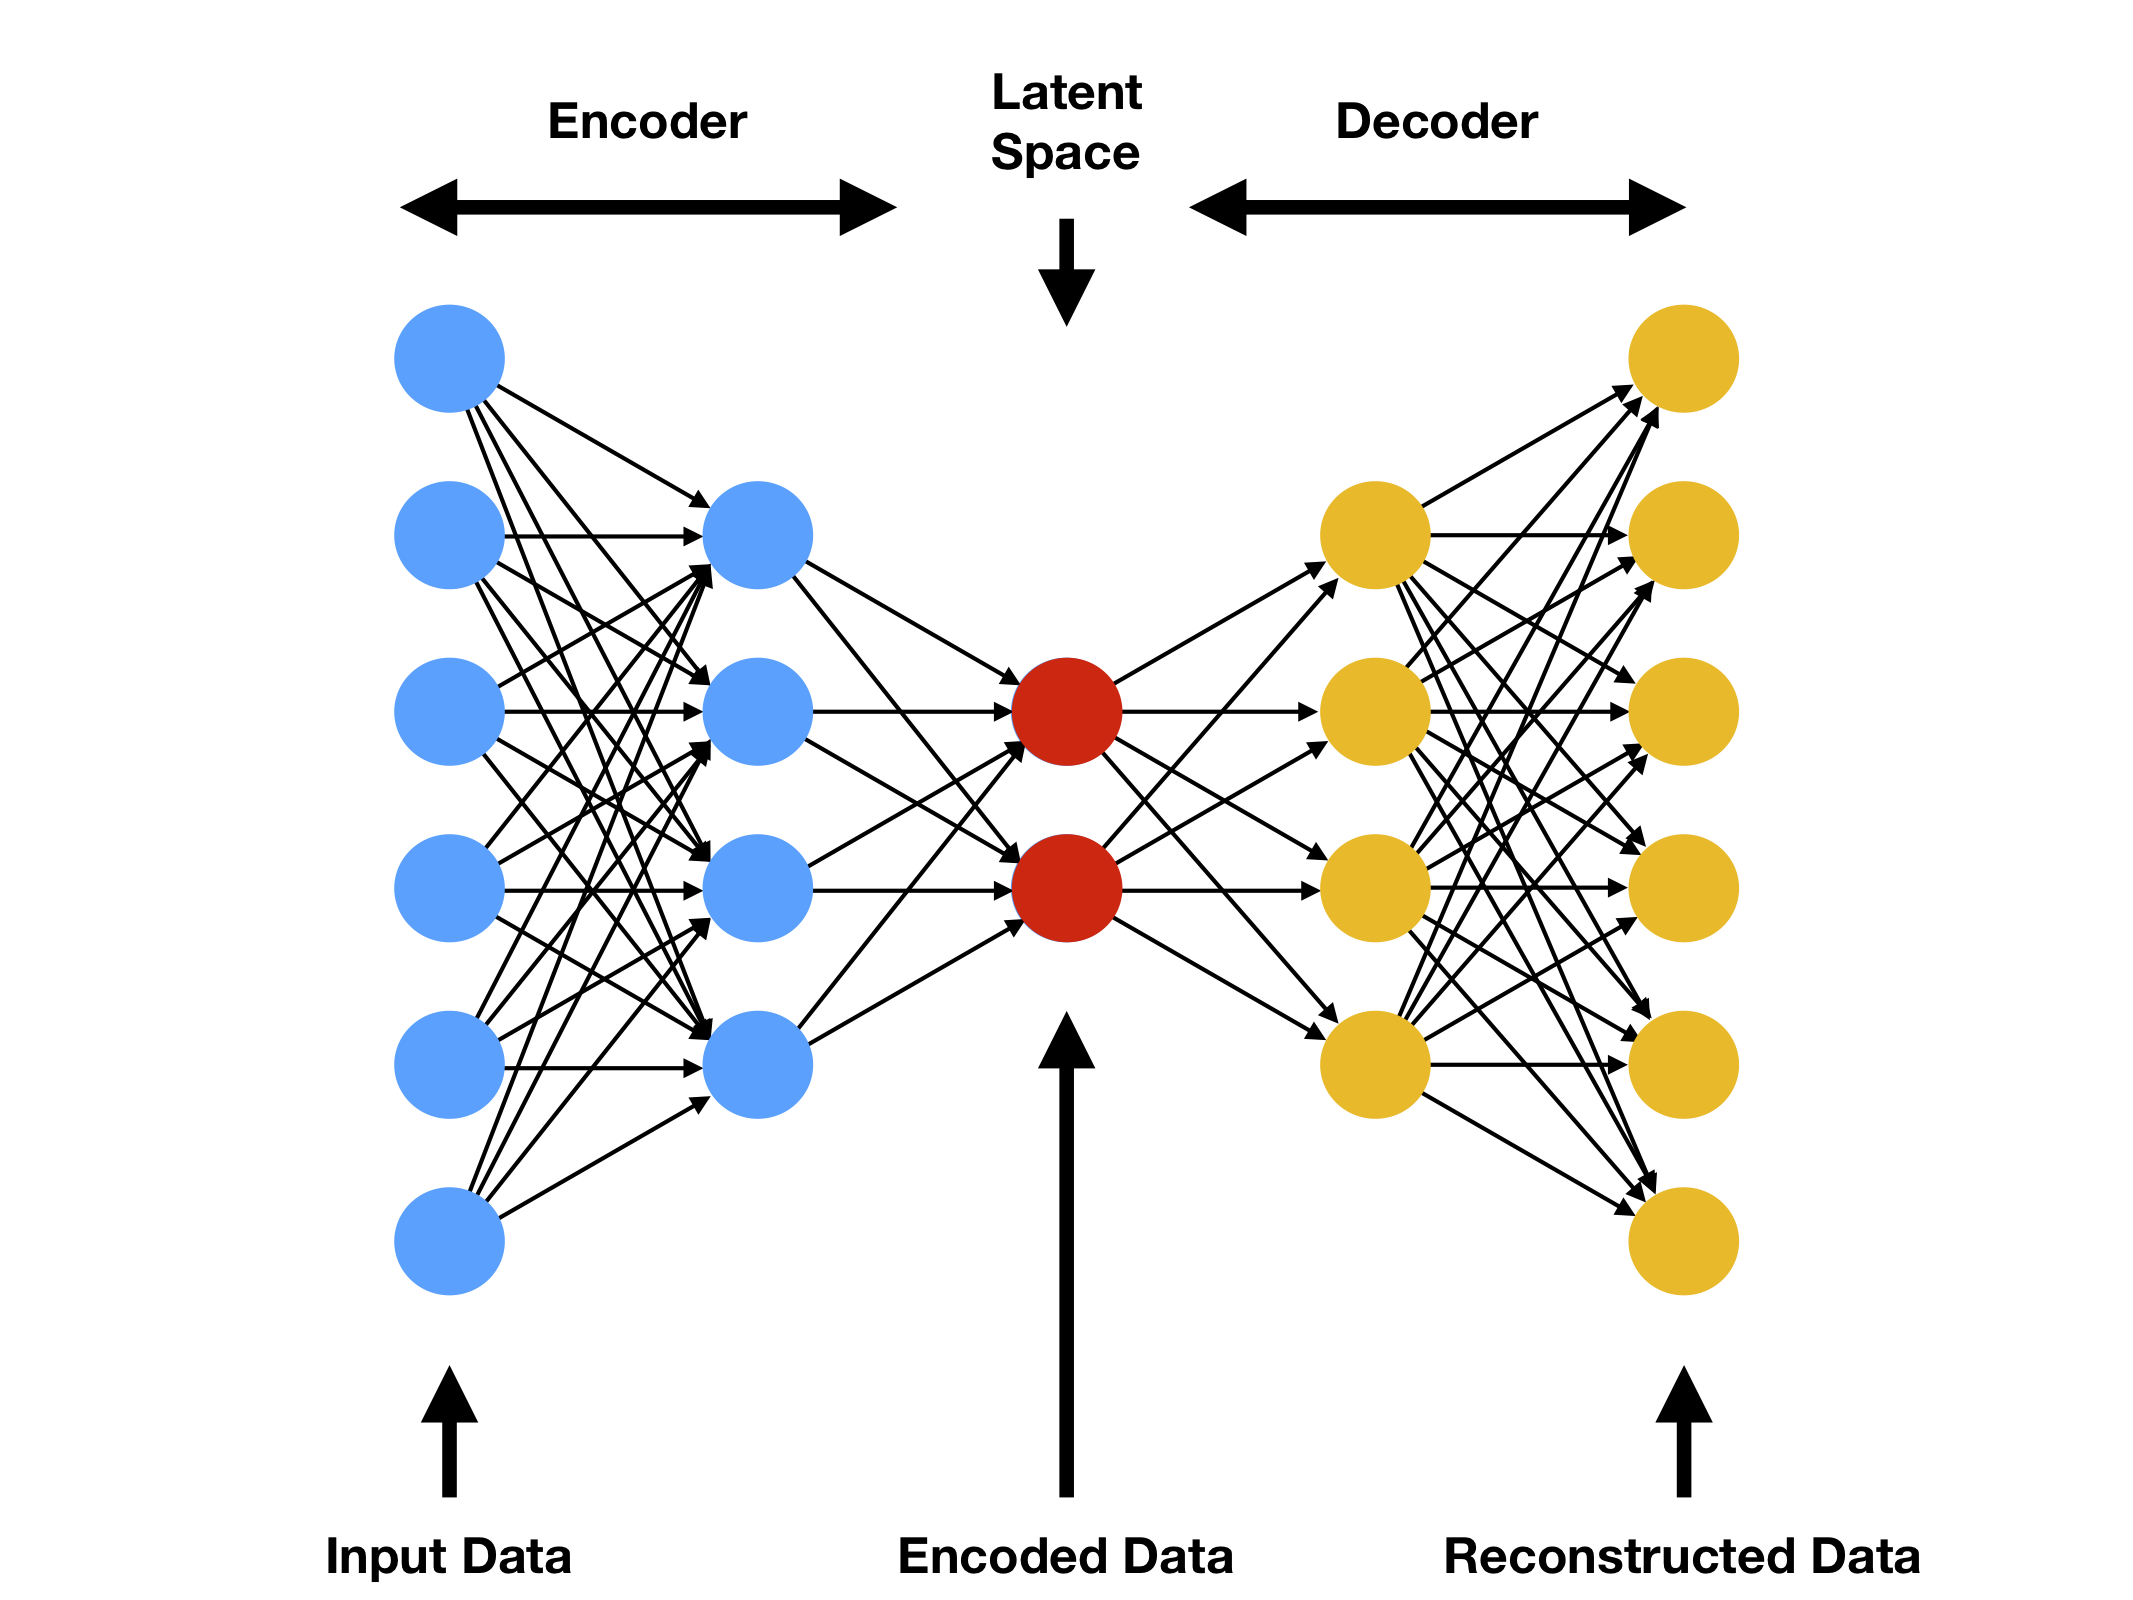
\includegraphics[width=0.8\textwidth]{doc_hw04/images/autoencoder.png}
    \caption{Arquitectura de un modelo de autoencoder}
    \label{fig:autoencoder}
\end{figure}

\subsection{\textit{Clustering}}

Ya a partir de las representaciones en un espacio de dimensiones reducido se procede a hacer la agrupación de los documentos para obtener grupos de tópicos relevantes. En este caso se realizaron pruebas con los algoritmos de \textit{Spectral Clustering}, \textit{Agglomerative Custering} y \textit{K-Means}. Sin embargo, a partir de los resultados presentados en \cite{DeepRepresentationClusteringTweets} y la posibilidad de recuperar los documentos más cercanos al centro del \textit{cluster} se decidió utilizar únicamente el algoritmo de \textit{K-Means}. De forma general, este algoritmo genera un número K de centroides aleatorios que agrupan los puntos (en este caso las representaciones de los documentos) más cercanos y los asocia a un \textit{cluster}. Posteriormente, y de forma iterativa, estos centroides se recalculan como la media de los puntos (o documentos) que agrupa el \textit{cluster} y vuelve a definir los \textit{clusters}. Vale la pena aclarar que un parámetro importante a ajustar en este algoritmo es el \textit{K} o el número de \textit{clusters}. Para esto se realizaron pruebas con distinto número de K y se evidencio la descripción (o \textit{keywords}) asociada a cada tópico para tomar esta decisión.

\subsection{\textit{Keywords Extraction}}

Finalmente, para poder describir el tópico (la agrupación o \textit{cluster} de documentos), se procedió a extraer las palabras que lo describen. Estos dan una idea de donde están concentrados los documentos más representativos del \textit{cluster}. De esta manera, se recuperó un número \textit{N} de documentos "relevantes", que son aquellos que se encuentran más cerca al centro del \textit{cluster}. Y, posteriormente, se extrajeron de esos documentos aquellos términos (o tokens) con mayor frecuencia dentro de esos documentos. Por último estos tópicos se presentan en el formato de \textit{wordcloud} para poder hacer más fácil su análisis.
